\documentclass[twocolumn, aps, rmp, amsmath, amssymb, nofootinbib, superscriptaddress, longbibliography, floatfix, table-of-contents, eqsecnum]{revtex4-1}

\usepackage[pdftex]{graphicx}
\usepackage{amssymb,amsmath}
\usepackage{color}

\newcommand{\bra}[1]{\langle#1|}
\newcommand{\ket}[1]{|#1\rangle}

\begin{document}

\title{Superconducting and Microwave qubits}
\maketitle

\section{Artificial atoms}

Qubits, the fundamental blocks of a quantum computer are designed by considering the lowest two energy levels of a quantum system. Based on the spacing between the energy levels, the quantum systems are classified into two types. The quantum harmonic oscillator type with equal spacing between the levels and the atomic type with unequal spacing between the levels. We illustrate these two cases in Fig.~\ref{fig:artificial_atom_energy_levels} where we show their corresponding energy level diagrams. This can be observed from the equations describing the energy levels of the respective systems,
\begin{align}
E_{n} &= (n+1/2) \hbar \omega \quad (\mathrm{Oscillator\,levels}) \nonumber \\ 
E_{n} &= -\frac{E_{0}}{n^{2}} \quad (\mathrm{Atomic\,levels})
\end{align}

To construct a qubit we should be able to use external fields to control and selectively drive a transition between only two energy levels in the system. Such a procedure is easy to achieve in atomic systems, but it is not possible to address only two levels in a quantum oscillator due to the harmonicity or equal energy spacing between the energy levels. On the other hand it is hard to work with individual natural atoms, mainly because of their size which makes their isolation and control very difficult. To overcome this disadvantage we need to develop new devices with quantum nature and anharmonic energy spectrum. Such devices are referred to as artificial atoms due to their similarity to natural atoms in the anharmonicity of the energy level spectrum.

\begin{figure}[!htbp]
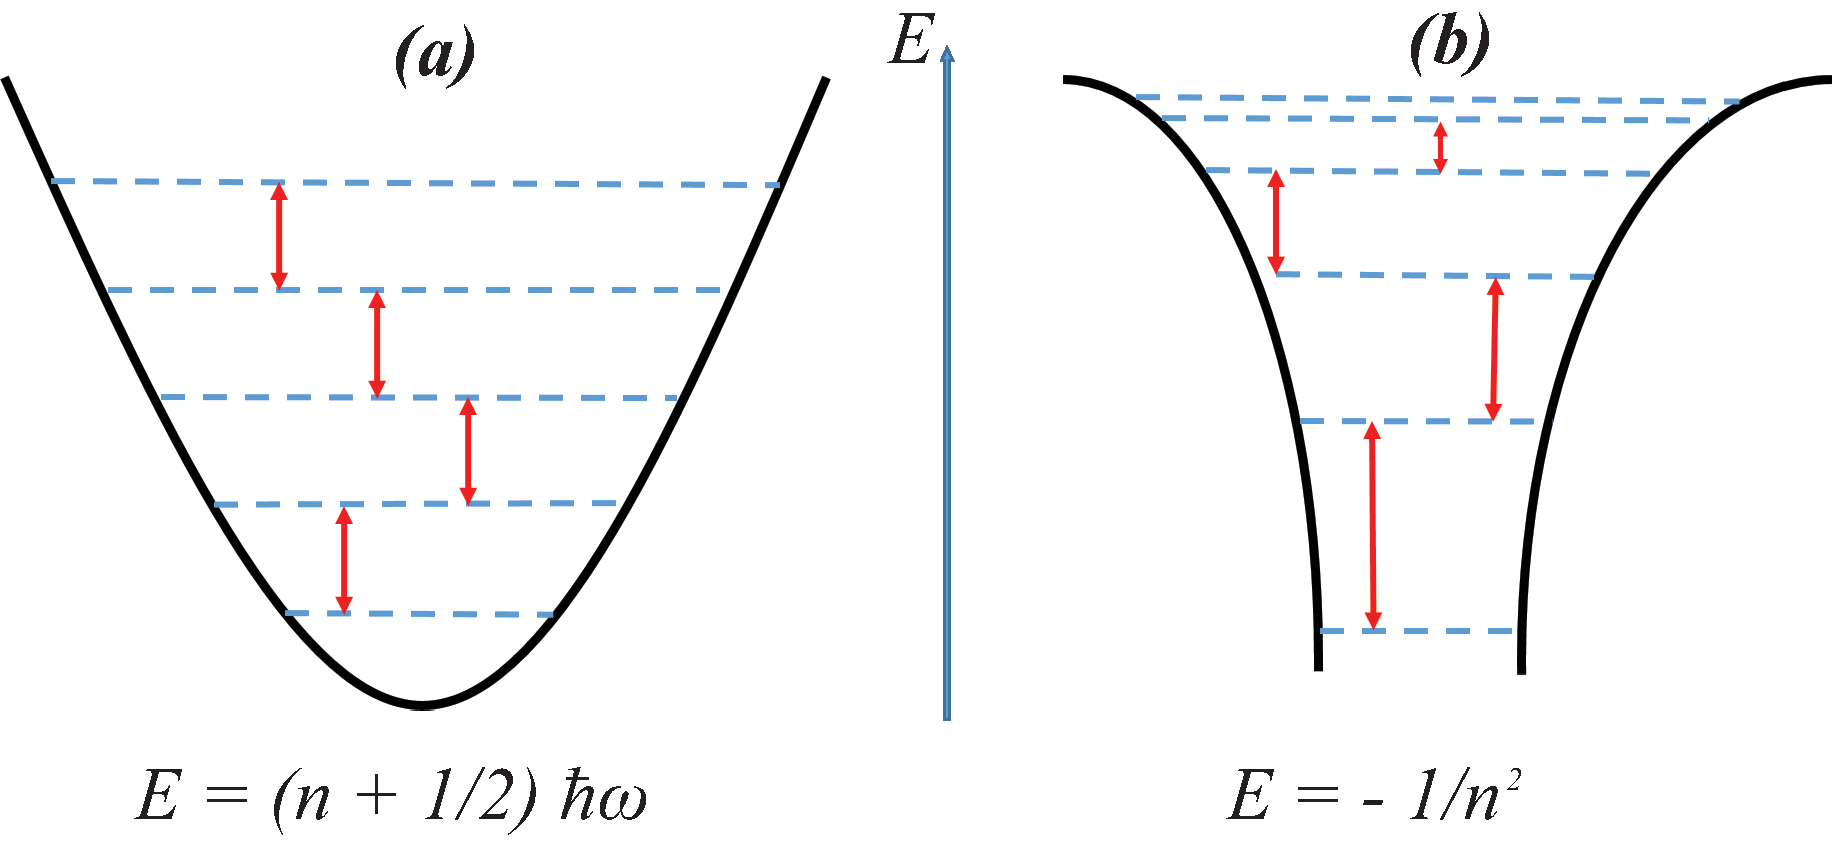
\includegraphics[width=0.475\textwidth]{artificial_atom_energy_levels}
\caption{The energy level of an (a) quantum oscillator and (b) atomic system.}\label{fig:artificial_atom_energy_levels}
\end{figure}

\section{Superconducting qubits}

One of the most widely used type of artificial atoms are the superconducting qubits \cite{bib:martinis1985energy, bib:shnirman1997quantum, bib:averin1998adiabatic, bib:devoret2004superconducting, bib:makhlin2001quantum} which are a class of nonlinear quantum circuits. An LC oscillator composed of an inductor $L$ and a capacitance $C$ is a typical example of a linear quantum circuit with equal spacing between the levels. By introducing a Josephson junction to the linear quantum circuit we can make it nonlinear with an anharmonic energy spectrum. For a better understanding of the superconducting qubits we would like to briefly explain the Josephson junction. A Josephson junction \cite{bib:josephson1974the} comprises of two bulk superconducting materials separated by a thin layer of an insulating material. In the superconducting phase the superconductors contain Cooper pairs which are composed of paired electrons. These Cooper pairs move from one superconducting layer to another through the insulating layer via quantum tunnelling. The quantum mechanical nature of Josephson junction is determined by two important energy scales. They are the Josephson coupling energy $E_{J}$ and the coulomb energy $E_{c}$. The ratio between these two energy scales determine the energy spectrum of the superconducting qubit. Hence we have three types of qubits {\it viz}, the voltage driven charge qubit \cite{bib:bouchiat1998quantum, bib:nakamura1999coherent}, the flux driven flux qubit \cite{bib:friedman2000quantum, bib:van2000quantum} and the current driven phase qubit \cite{bib:martinis2002rabi}. 

\subsection{Charge qubits}

A nonlinear quantum circuit driven by voltage is referred to as a charge qubit. The Hamiltonian of a charge qubit is,
\begin{align}
\hat{H} = \frac{q^{2}}{2C} - E_{J} \cos \left( \frac{2e}{\hbar} \phi \right)
\label{circuitHamiltonian}
\end{align}
Here $q$ is the charge in the superconducting system and $\phi$ is the flux in the qubit. The total capacitance of the circuit is given by $C$ and $E_{J}$ is the Josephson energy. The Hamiltonian in (\ref{circuitHamiltonian}) can be rewritten as,
\begin{align}\label{eq:charge_qubit_hamiltonian}
H = 4E_{c} (\hat{n} - n_{g})^{2} - E_{J} \cos (\hat{\phi}) .
\end{align}

The variables $q$ and $\hat{\phi}$ are canonically conjugate and satisfy the commutation relation,
\begin{align}
[ \hat{\phi},\hat{q} ] = i \hbar
\end{align}
In a truncated charge basis the Hamiltonian is,
\begin{align}
\hat{H} &= 4 E_{c} \sum_{n = -N}^{N} (n - n_{g})^{2} \ket{n}\bra{n}\nonumber\\
&- E_{J} \sum_{n = -N}^{N-1} \ket{n+1}\bra{n} + \ket{n}\bra{n+1}.
\end{align}

The energy eigenstates are the charge states $\ket{n}$ and hence these qubits are referred to as the charge qubit. In general the charge qubit \cite{bib:bouchiat1998quantum, bib:nakamura1999coherent} is operated in the region $E_{J}/E_{C} \approx 1$. The charge qubits are highly sensitive to noise except at particular working points referred to as sweet spots. But it is experimentally hard to control the voltage and current such that the qubit is maintained at these desired working conditions. To overcome this a special design of charge qubit known as transmission line shunted plasma oscillation qubit or transmon \cite{bib:koch2007charge} with $E_{J}/E_{C} \gg 1$ was suggested. The transmon is highly robust to external to noise in comparison with the charge qubit. But the energy levels become more and more harmonic i.e., equal spaced as we move away from the region $E_{J}/E_{C} \approx 1$. Thus the charge qubits are designed by giving considerations to the trade-off between the robustness to external noise and the anharmonicity between the levels. The twenty qubit prototype quantum computer developed by IBM uses transmon type superconducting qubits \cite{bib:gambetta2017building}. 

\subsection{Flux qubits}

The flux qubit is popularly known as the RF SQUID (Radio Frequency Superconducting QUantum Interference Device) and works in an AC current. This qubit can be considered as the magnetic analogue of the Charge qubit. In a charge qubit the Josephson junction is driven by a capacitor, but in a flux qubit, a superconducting transformer circuit generates the flux which drives the circuit. The Hamiltonian of the circuit is,
\begin{align}
\hat{H} = \frac{q^{2}}{2 C_{J}} + \frac{\phi^{2}}{2 L} - E_{J} \cos \left( \frac{2e}{\hbar}(\phi - \phi_\mathrm{ext}) \right).
\end{align}
Here we can observe that there are three energy scales namely $E_{J}$, $E_{c} = (2e)^{2} / 2C$ and $E_{L} = \phi_{0}^{2} /2L$. The quantum properties of the qubit depends on the interplay between these parameters. The Cooper pairs in a flux qubit are confined to a double well potential. The variables of $Q$ and the total magnetic flux $\Phi$ are the conjugate variables and they satisfy the commutation relation,
\begin{align}
[\hat{Q},\hat\Phi] = i \hbar.
\end{align} 
The flux qubits are very robust to charge noise \cite{bib:you2005fast} and hence they have very high decoherence time which makes them one of the most preferred qubits in the construction of quantum computers. The quantum computing device developed by D-Wave uses flux qubits \cite{bib:harris2018phase}.

\subsection{Phase qubits}

The current driven superconducting qubits are referred to as phase qubits \cite{bib:martinis2002rabi}. They are commonly known as DC SQUID and operate at very high values of $E_{J}/E_{c}$.

The Hamiltonian of a phase qubit is,
\begin{align}
\hat{H} = E_{c} p^{2} - I \phi_{0} \delta - I_{0} \phi_{0} \cos \delta,
\label{eq:phase_qubit_hamiltonian}
\end{align}
where $\delta$ is the gauge invariant phase difference operator and the charge on the capacitor is $2pe$. These operators are conjugate variables and they satisfy the commutation relation $[\delta, p] = i \hbar$. In the phase qubit the Cooper pairs experience a washboard potential. Since the decoherence time of the phase qubits are very less in comparison with the flux and the charge qubits, they are not that widely used.

\begin{figure}[!htbp]
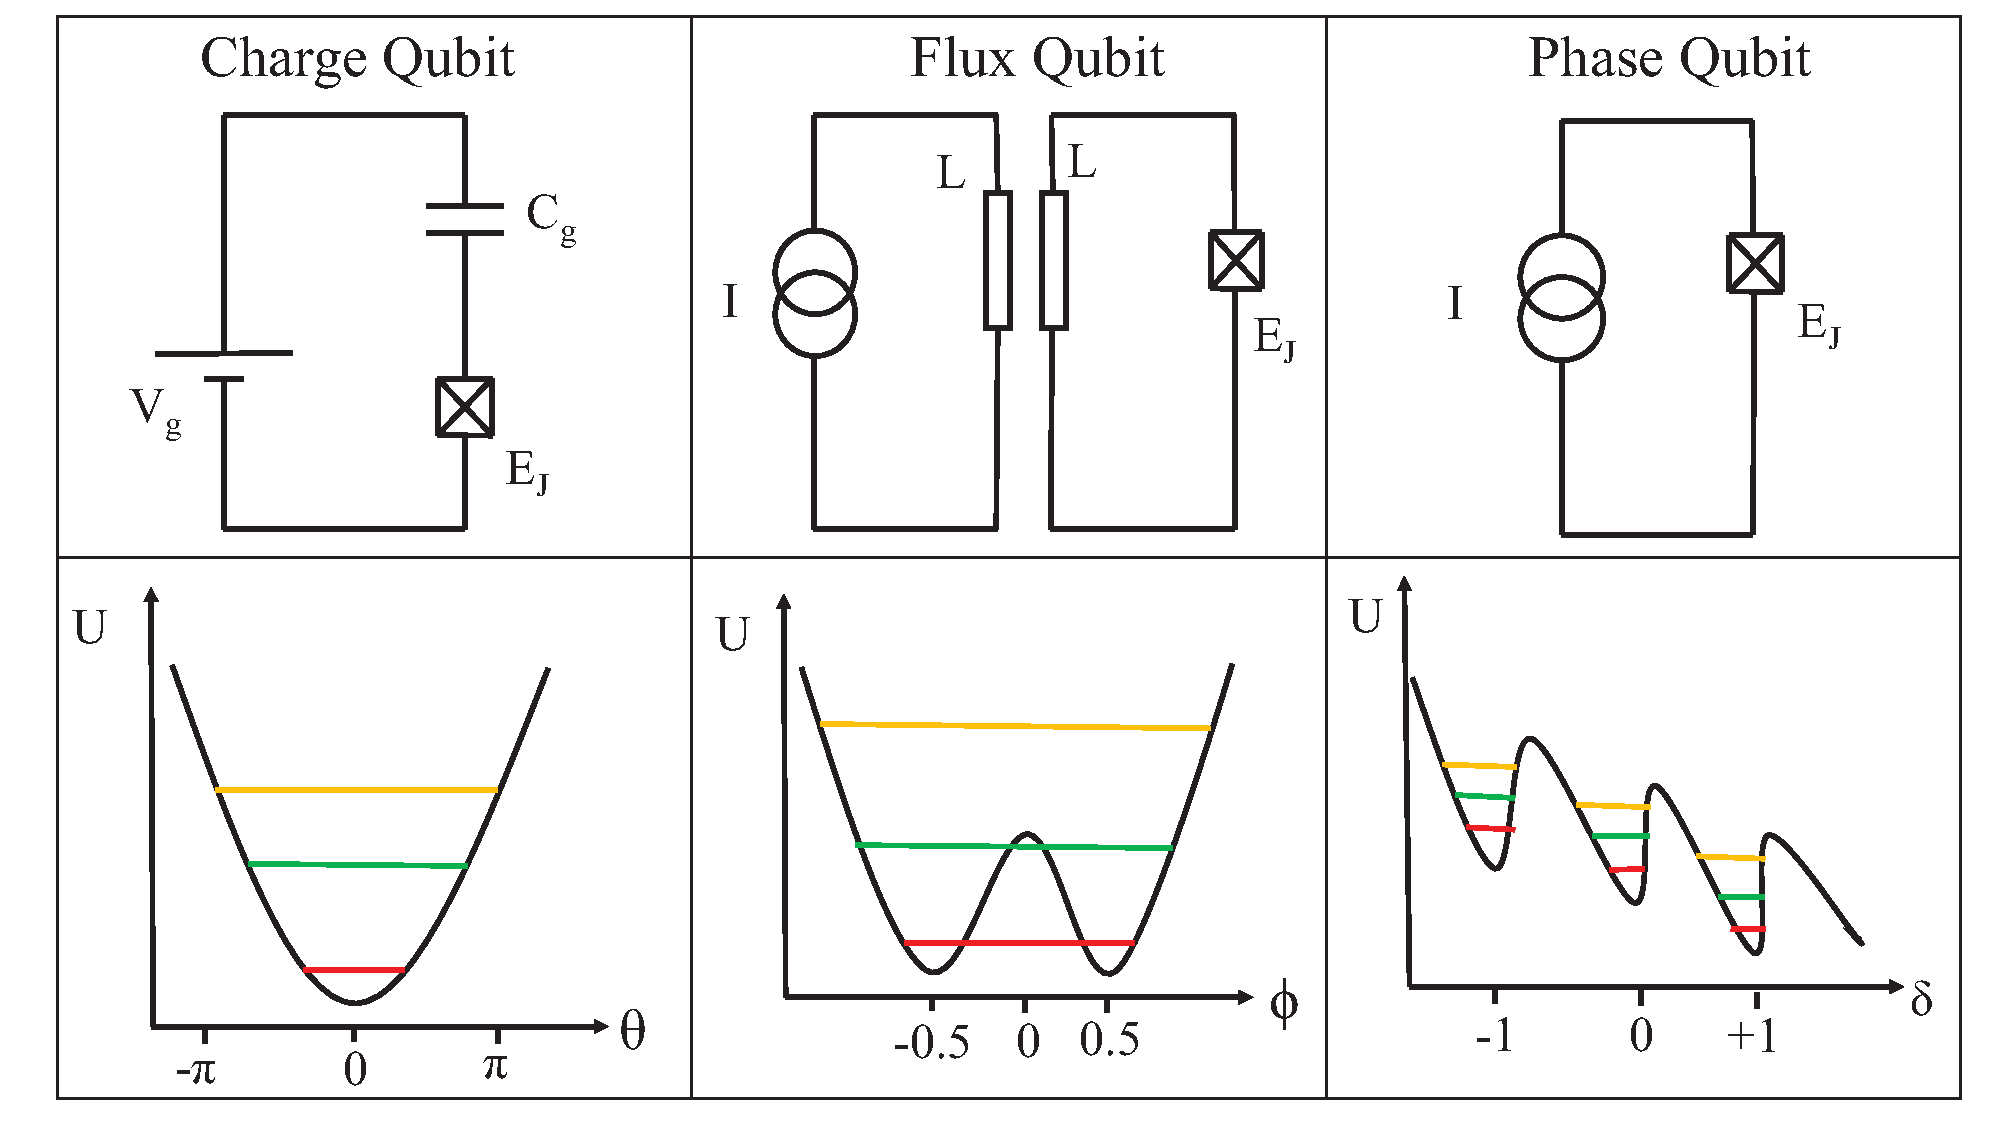
\includegraphics[width=0.475\textwidth]{superconducting_qubits}
\caption{Simplified circuits of the different kinds of superconducting qubits, namely the charge qubit, flux qubit and phase qubit. Below each circuit are their respective energy level diagrams.} 
\end{figure}

\section{Flying qubits}

A quantum computer will be made up of several superconducting qubits and a quantum operation will mostly involve more than one qubit. Hence it is essential to find ways to transfer the information from one set of superconducting qubits to another. While transferring the information we need to keep in mind that its quantum nature should be preserved. This essentially means we need to find a different kind of qubit which can carry information from one place to another and interacts weakly with the other qubits and the environment. It is well known that photons can move from one place to another and they interact very weakly with each other and the environment. They can be made into qubit systems by using their horizontal and vertical polarisation degrees of freedom as two levels of the system. The photonic qubits useful to carry information should have frequency which is equal to the energy difference between the qubit levels. For a superconducting qubit the energy difference is very small and hence the frequency of the optical qubits will correspond to microwaves whose wavelength lies in the range from 100$\mu$m and 1m.

The information transfer between the different superconducting qubits is achieved using a resonator which acts as a quantum data bus. A simple resonator is an LC circuit which can support only one frequency mode, but a waveguide resonator can support multiple modes. In general the transmission line circuits used in the quantum non-linear electric circuits are in the form of coplanar waveguides. These waveguides are engineered to handle a particular set of frequencies and it is also to produce transmission lines of tuneable frequencies. The tuneable resonators are very important in quantum optics and are useful in implementing controllable coupling between different quantum elements and also in shaping the wave packets of photons. 

In cavity quantum electrodynamics the interaction of a natural atom with an optical photon in the visible wavelength is studied. Similarly, the interaction between the quantum non-linear electrical circuit and the microwave photon is investigated in circuit quantum electrodynamics. The coupling strength between a natural atom and visible light photon is fixed and an atom couples weakly with the photon \cite{bib:raimond2001manipulating}. Meanwhile the coupling strength between a superconducting qubit and microwave can be changed by engineering the parameters of the qubit and resonator and we can have strong and ultra strong coupling between the qubit and the photons \cite{bib:wallraff2004strong}. Further the coupling between the atom and the photon can be tuned during the course of an experiment. Several quantum optics components like mirrors, beamsplitters, circulators and switches can also be designed based on the quantum electric circuits.

\begin{figure}[!htbp]
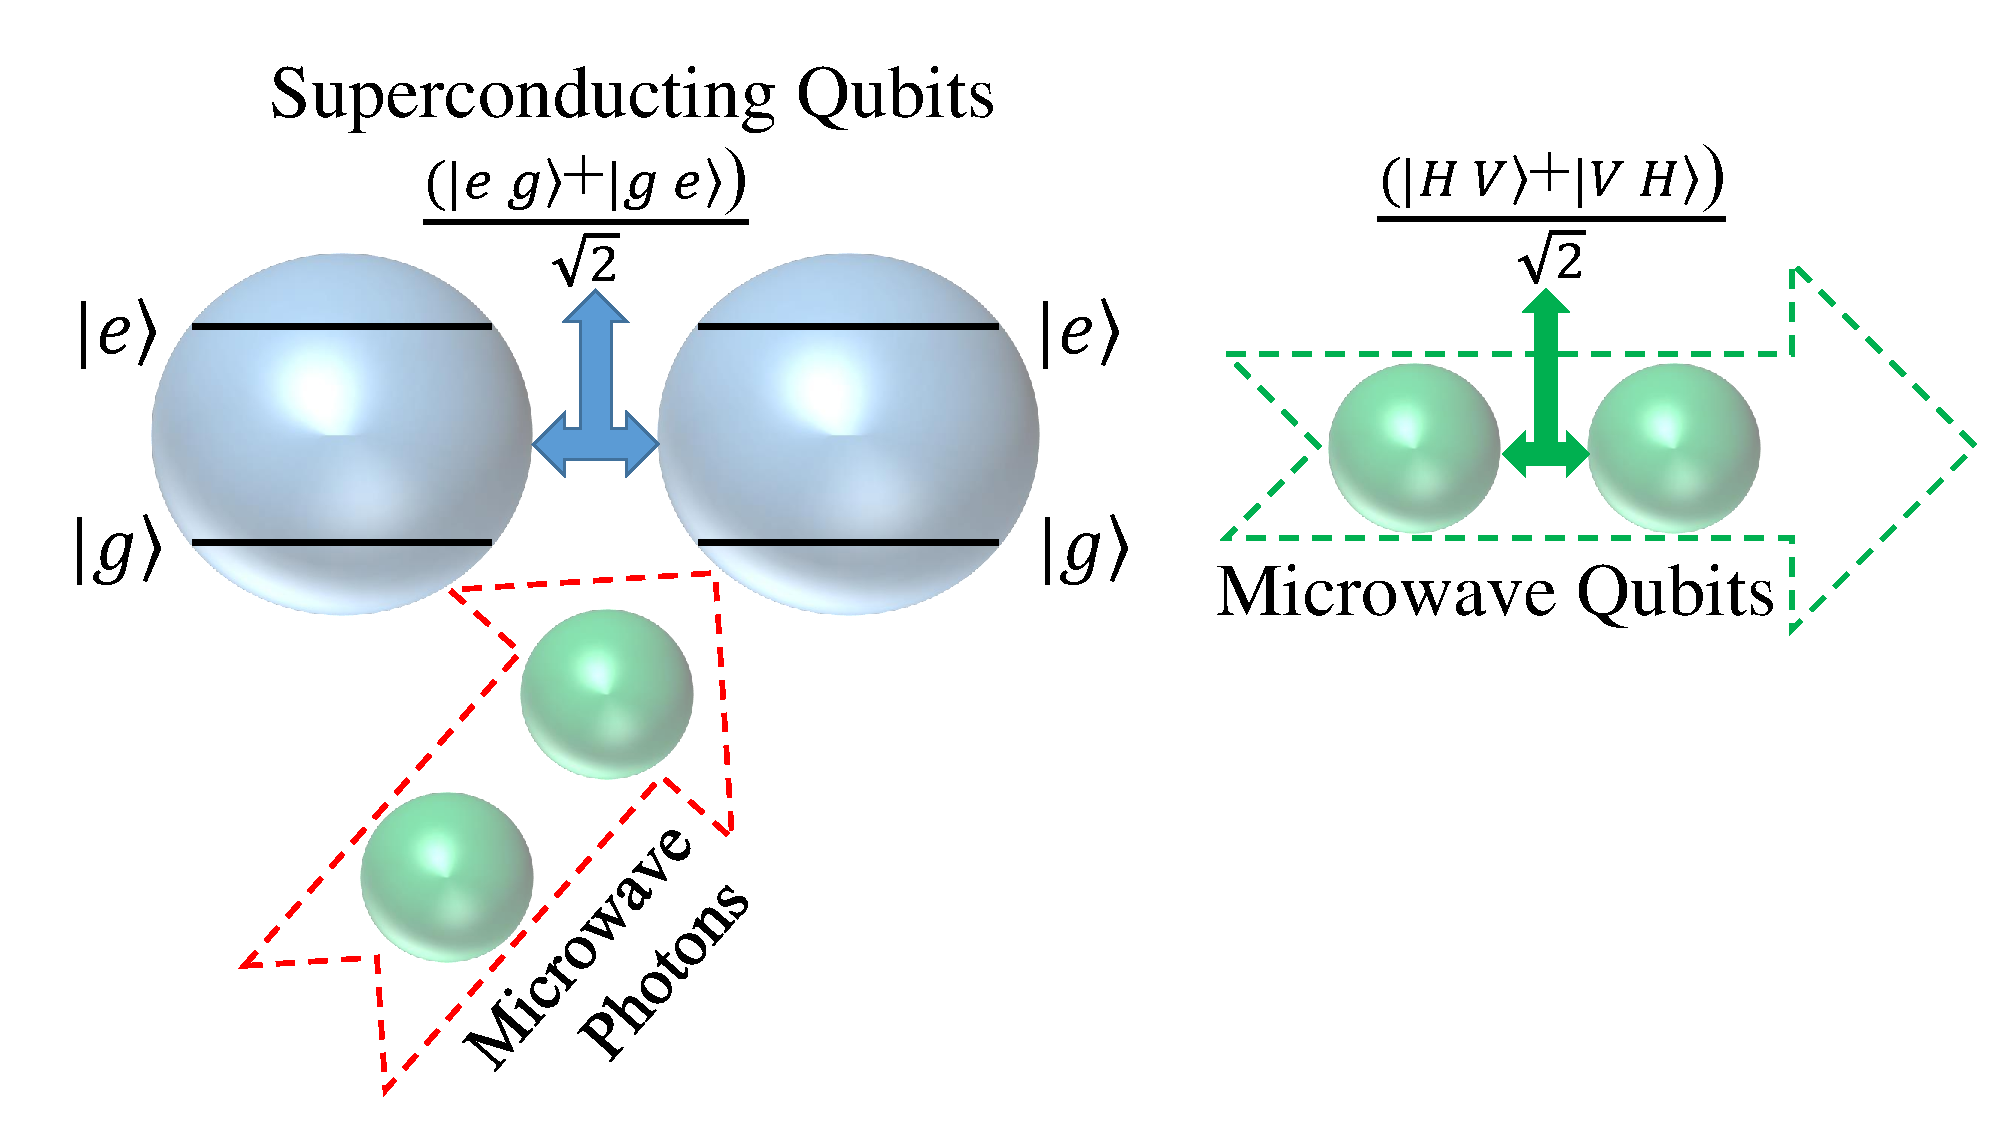
\includegraphics[width=0.475\textwidth]{microwave_qubits}
\caption{A schematic sketch of the interaction between superconducting qubits and microwave qubits is shown. The superconducting qubits are in the entangled state $(\ket{e g} + \ket{g e }/\sqrt{2}$ where $\ket{g}$ and $\ket{e}$ are the ground and excited states of the superconducting qubits. These superconducting qubits are subjected to interact with the flying qubits which is the microwave qubit (red dashed arrow) in this case. The photons get entangled and the output state of the photons is $(\ket{H V} + \ket{V H})/\sqrt{2}$, where $\ket{H}$ and $\ket{V}$ are the horizontal and vertical polarisation modes.}\label{fig:microwave_qubits}
\end{figure}

\section{Quantum gates based on superconducting qubits}

The qubits form the elemental unit of a quantum computer, but the operational unit is the quantum logic gate which is a fundamental quantum circuit made of a specific number of qubits. To use the superconducting qubit for applications in quantum computing we need to design quantum gates based on them and several investigations have been carried out on them \cite{bib:blais2004cavity, bib:chow2011simple, bib:chow2013microwave}. Below we give a brief description of single and two qubit quantum gates based on superconducting qubits.

\subsection{Single qubit quantum gates}

A single superconducting qubit which is coherently controlled using microwave can be used as a quantum gate. Let us consider a cavity with a resonance frequency $\omega_{r}$ and drive frequency $\omega_{d}$, where the difference $\Delta_{r} = \omega_{r} - \omega_{d}$ is the detuning between the cavity and the drive. When $\omega_{d} \approx \omega_{r}$ one can read the state of a superconducting qubit using microwaves. But when $\omega_{d} = \omega_{q} \ll \omega_{r}$ the microwave can be used to perform gate operations on the qubit without measuring its state.

The system comprising of a superconducting qubit and a microwave can be described using the Jaynes-Cummings Hamiltonian,
\begin{align}
\hat{H} = \Delta _{r} \hat{a}^{\dag} \hat{a} - \frac{\Delta_{q}}{2} \hat\sigma_{z} + g (\hat{a}^{\dag} \hat\sigma_{-} + \hat{a} \hat\sigma_{+}) + \xi(t) (\hat{a}^{\dag} + \hat{a}),
\label{eq:driven_jc_hamiltonian}
\end{align}
where $\hat{a}^{\dag}$ ($\hat{a}$) is the creation (annihilation) operator corresponding to the microwave photon and $\sigma_{+} (\sigma_{-})$ is the spin raising (lowering) operator. The factors $\Delta_{r} = \omega_{r} - \omega_{d}$ and $\Delta_{q} = \omega_{q} - \omega_{d}$ are the detuning parameters. The factor $g$ is the coupling between the microwave photon and the qubit and $\xi(t)$ is envelope of the microwave pulse. The effective Hamiltonian corresponding to Eq.~(\ref{eq:drivenjchamiltonian}) is,
\begin{align}
\hat{H}_\mathrm{eff} &= \left( \Delta_{r} + \frac{g^{2}}{\Delta} \hat\sigma_{z} \right) \hat{a}^{\dag} a - \frac{1}{2} \left(\Delta_{q} - \frac{g^{2}}{\Delta} \right) \hat\sigma_{z} \nonumber\\
&+ \xi(t) (\hat{a}^{\dag} + \hat{a}) - \frac{g \xi(t)}{\Delta} \hat\sigma_{x}
\end{align}

To perform a X-gate using a superconducting qubit which performs a pure X-rotation we choose a drive frequency $\omega_{d} = \omega_{q} - (2 \bar{n} + 1) g^{2}/\Delta$, which causes the $\sigma^{z}$ term to disappear and leaves us with a pure $\sigma^{x}$ rotation. Using a phase shifted drive $H^{d}(t) = \xi(t) i (a^{\dag} - a)$ one might obtain purely $\sigma^{y}$ rotation which will lead to a the construction of a Y-gate. Finally we note that using a drive $\omega_{d} = \omega_{q} - (2 \bar{n} + 1) g^{2}/\Delta - 2 g \xi(t)/\Delta$ we will be able to construct an Hadamard gate. 

\subsection{Two-qubit quantum gates}

Quantum gates based on two qubits can be realised in many different ways. But in terms of their construction and operation they can be divided into two classes. In the first class of quantum gates the superconducting qubits can be tuned over a wide range of frequencies. A good example of this is the iSWAP gate in which two cooper pair boxes are coupled via a transmission line resonator. In the rotating frame of reference the effective of the Hamiltonian of the system is,
\begin{align}
\hat{H}_\mathrm{eff} &= \frac{g^{2}}{\Delta} \left( \hat{a}^{\dag} \hat{a} + \frac{1}{2} \right) (\hat\sigma_{z,1} + \sigma_{z,2}) \nonumber\\
&- \frac{g^{2}}{\Delta} (\hat\sigma_{+,1} \hat\sigma_{-,2} + \hat\sigma_{+,2} \hat\sigma_{-,1}).
\end{align}
The parameters of the two qubits can be adjusted by tuning their flux. The interaction between the two qubits can be turned on and off by tuning the qubits in and out of resonance with each other. The advantage of the first class of quantum gates is that they can be operated in a region where the frequency of the two qubits differ from each other and when the interaction between them is very high. But the disadvantage is that these qubits are sensitive to flux noise and hence they require extra flux bias lines for tuning them properly.

The second class of quantum gates are built up of superconducting qubits with fixed frequencies and are driven by microwaves. The Cross-resonance gate, the bSWAP or Bell-Rabi gate and the MAP gate belong to this class. The effective Hamiltonian of the Cross-resonance gate is 
\begin{align}
\hat{H}_\mathrm{eff} = - \left( \frac{\tilde{\omega}_{1} - \tilde{\omega}_2}{2} \right) \hat\sigma_{z,1} + \frac{\Omega(t)}{2} \left(\hat\sigma_{x,1} - \frac{J}{\Delta_{12}} \hat\sigma_{z,1} \hat\sigma_{x,2} \right),
\end{align}
where $\tilde{\omega}_{1} = \omega_{1} + J^{2}/\Delta_{12}$ and $\tilde{\omega}_{2} = \omega_{2} - J^{2}/\Delta_{12}$ and $\Delta = \omega_{1} -\omega_{2}$. The factors $\omega_{1}$ and $\omega_{2}$ are the frequencies of the first and the second qubit and $\Delta_{12}$ is the detuning. The first qubit is rotating at a frequency of $\frac{\tilde{\omega_{1}} - \tilde{\omega_{2}}}{2}$ around the Z-axis with a little shift in the X direction and hence we have an X-gate. Similarly we can construct a microwave-activated c-phase (MAP) gate using two transmons. The system of two transmons are modelled using a system of two coupled Duffing oscillators. The effective Hamiltonian in the two qubit space reads,
\begin{align}
\hat{H}_\mathrm{eff} &= - \frac{1}{2} \left( \omega_{01} - \frac{\zeta}{2} \right) \hat\sigma_{z,1} - \frac{1}{2} \left( \omega_{10} - \frac{\zeta}{2} \right) \hat\sigma_{z,2} \nonumber\\
&+ \frac{\zeta}{4} \hat\sigma_{z,1} \hat\sigma_{z,2}. 
\end{align}

Through this Hamiltonian we can realize a c-phase quantum gate with a gate time $t = 514$ns and high fidelity. The second class of quantum gates have a longer coherence time since the superconducting qubits can be parked at the sweet spots of coherence where the effect of noise on the qubits are much lower. But the control of the qubits are much harder since we need to maintain them at the same values of qubit parameters for an extended period of time.

\section{Quantum transducers}

The realisation of quantum computers as well as quantum communication relies very much on the development of a quantum network. Here the nodes of a network might be made of either logic gates which perform quantum operation or the nodes might correspond to different quantum computers. One recent possibility is the formation of a network of quantum satellites performing quantum communication. Such networks will form the basis of quantum internet. One of the major requirement for the network is the transfer of quantum information with high fidelity between the different nodes of such a network. 

The fundamental unit of a quantum computer is a qubit and due to scalability requirements, superconducting qubits are the most widely used form of qubits. It is well known that the energy-level spacing in a superconducting qubits corresponds to the microwave regime. Hence to control and transfer information from a superconducting qubit one might need to use microwave photons. In principle we can use microwave photons to transfer information from one node to another, but such a transmission process is extremely lossy. Also such processes have very high technical requirements like the design of specialised waveguides made of Niobium and being maintained at extremely low temperatures. Hence it is not feasible to use microwave photons for long distance transfer of quantum information. Meanwhile it is well known that photons in the visible spectrum can be transmitted easily using optical fibres. To convert the microwave photons to optical photons we can use a quantum transducer. A sketch of a typical design for a quantum transducer is shown in Fig.~\ref{fig:quantum_transducer} through a flow chart diagram. The quantum computer is made up of superconducting qubits which feeds the quantum information to microwave qubits. The microwave qubits are then connected to the optical qubits in the visible spectrum through a three level quantum system which can couple at both microwave and optical frequencies. These steps should be reversible and hence it should be possible to convert the optical qubits into the microwave qubits at the receiving end. 

There are several proposals for quantum transducers in existence and they can be classified into two major classes:
\begin{itemize}
	\item Opto-mechanical \cite{bib:rabl2010quantum, bib:barzanjeh2011entangling, bib:bochmann2013nanomechanical, bib:didier2014quantum, bib:schuetz2015universal, bib:shumeiko2016quantum, bib:stannigel2010optomechanical}.
	\item Spin ensembles \cite{bib:imamouglu2009cavity, bib:blum2015interfacing}
\end{itemize}

In the opto-mechanical quantum transducer as the name suggests combines optical components with a nano-mechanical resonator and converts the microwave photon into a phonon (acoustic) mode. The acoustic mode is then transmitted through waveguides. Since we need to fabricate wave guides with very high precision to transmit phonon modes, this scheme is not suitable for communicating between two quantum computers. A coupling of this phonon mode to the optical photon mode in the visible region was suggested to enable the transfer of quantum information over long distance. The Hamiltonian of an opto-mechanical quantum transducer which converts a microwave photon to optical photon using an intermediate nano-mechanical resonator reads,
\begin{align}
\hat{H} &= \hbar \omega_{1} \, \hat{a}_{1}^{\dag} \hat{a}_{1} + \hbar \omega_{2} \, \hat{a}_{2}^{\dag} \hat{a}_{2} \nonumber\\
&+ \hbar \Omega \, \hat{b}^{\dag} \hat{b} + \hbar \, g \, (\hat{b}+\hat{b}^{\dag}) (\hat{a}_{2}^{\dag} \hat{a}_{1} + \hat{a}_{1}^{\dag} \hat{a}_{2}),
\end{align}
here $\omega_{1}$ $(\omega_{2})$ is the frequency of the microwave (optical) photon and $\Omega$ is the phonon frequency. The operators $\hat{a}_{1}$ ( $\hat{a}_{1}^{\dag}$) and $\hat{a}_{2}$ ($\hat{a}_{2}^{\dag}$) denotes the annihilation (creation) operators corresponding to the microwave and optical photons respectively. Meanwhile $\hat{b}^{\dag}$ ($\hat{b}$) denotes the phonon creation and annihilation operators corresponding to the phonons. The factor $g$ is the coupling strength between the microwave, phonon and photon mode. This design of quantum transducer is widely preferred since the optical photons in the visible spectrum can be transmitted over long distance using optic fibres. But the scheme requires two intermediate conversions which decreases the overall efficiency of the process.

The spin ensemble based quantum transducer is an alternative to the opto-mechanical quantum transducer. In this scheme an ensemble of spins interact with the microwave qubits via magnetic dipole coupling strength, while the superconducting qubits interacts via electric dipole coupling with the microwave coupling. The Hamiltonian of such a design is as follows,
\begin{align}
\hat{H} = \hat{H}_{\mathrm{mw}} + \hat{H}_{\mathrm{spin}} + \hat{H}_{\mathrm{opt}},
\end{align}
where the various parts of the Hamiltonian are as follows,
\begin{align}
\hat{H}_{\mathrm{mw}} &= \hbar \omega_\mathrm{sq} \hat\sigma_\mathrm{sq}^{\dag} \hat\sigma_\mathrm{sq} + \hbar \omega_{\mu} \hat{a}^{\dag} \hat{a} + \hbar g_{\mu} (\hat{a}^{\dag} \hat\sigma_\mathrm{sq} + \hat{a} \hat\sigma_\mathrm{sq}^{\dag}),\nonumber \\
\hat{H}_{\mathrm{spin}} &= \hbar g_{s} (\hat\sigma_\mathrm{ba}^{\dag} \hat\sigma_\mathrm{ba} + \hat\sigma_\mathrm{bs}^{\dag} \hat\sigma_\mathrm{bs}), \nonumber\\
\hat{H}_{\mathrm{opt}} &= \hbar g_{ab} (\hat\sigma_\mathrm{ba}^{\dag} \hat{c} + \hat{c}^{\dag} \hat\sigma_\mathrm{ba}).
\end{align}

The factors $\omega_{sq}$ is the frequency of the superconducting qubit, and $\sigma_{sq}^{\dag}$ and $\sigma_{sq}$ are the raising and lowering operators corresponding to the superconducting qubits. The frequency of the microwaves is given by $\omega_{\mu}$ and the $a^{\dag}$ and $a$ are the creation and annihilation operator corresponding the microwave photons. The factor $g_{s}$ is the coupling between the interaction between the various levels of the spin and $\sigma_{ba}$ and $\sigma_{bs}$ are the spin operators corresponding to the transition between the levels $a$, $b$ and $s$. Finally the coupling strength of the spin interaction with the photon is denoted by $g_{ab}$ and $c^{\dag}$ ($c$) is the creation (annihilation) operator corresponding to the photon. Again this process is also a two step process which is in addition beset with problems of inhomogenous line broadening. Design of a high fidelity quantum transducer is still an open problem in the field of quantum technology. 

\begin{figure}[!htbp]
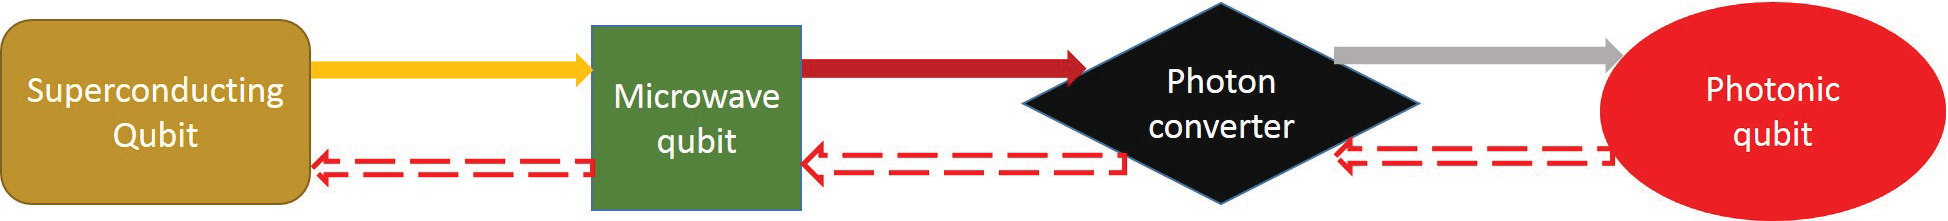
\includegraphics[width=0.475\textwidth]{quantum_transducer}
\caption{A block diagram of the quantum transducer is given in the figure above. The quantum computer made up of the superconducting qubit couples with the microwave qubit. The microwave qubit and the photonic qubit are coupled by a three level system in which the energy difference between the levels correspond to both microwave and visible optical frequencies. The thick arrows denote the forward process which is need to convert the microwave to the optical frequencies and the dashed arrows represent the reverse process which is needed at the receiving end to convert the optical frequency to a microwave frequency and feed the information to another set of quantum computer.}\label{fig:quantum_transducer}
\end{figure}

\begin{figure}[!htbp]
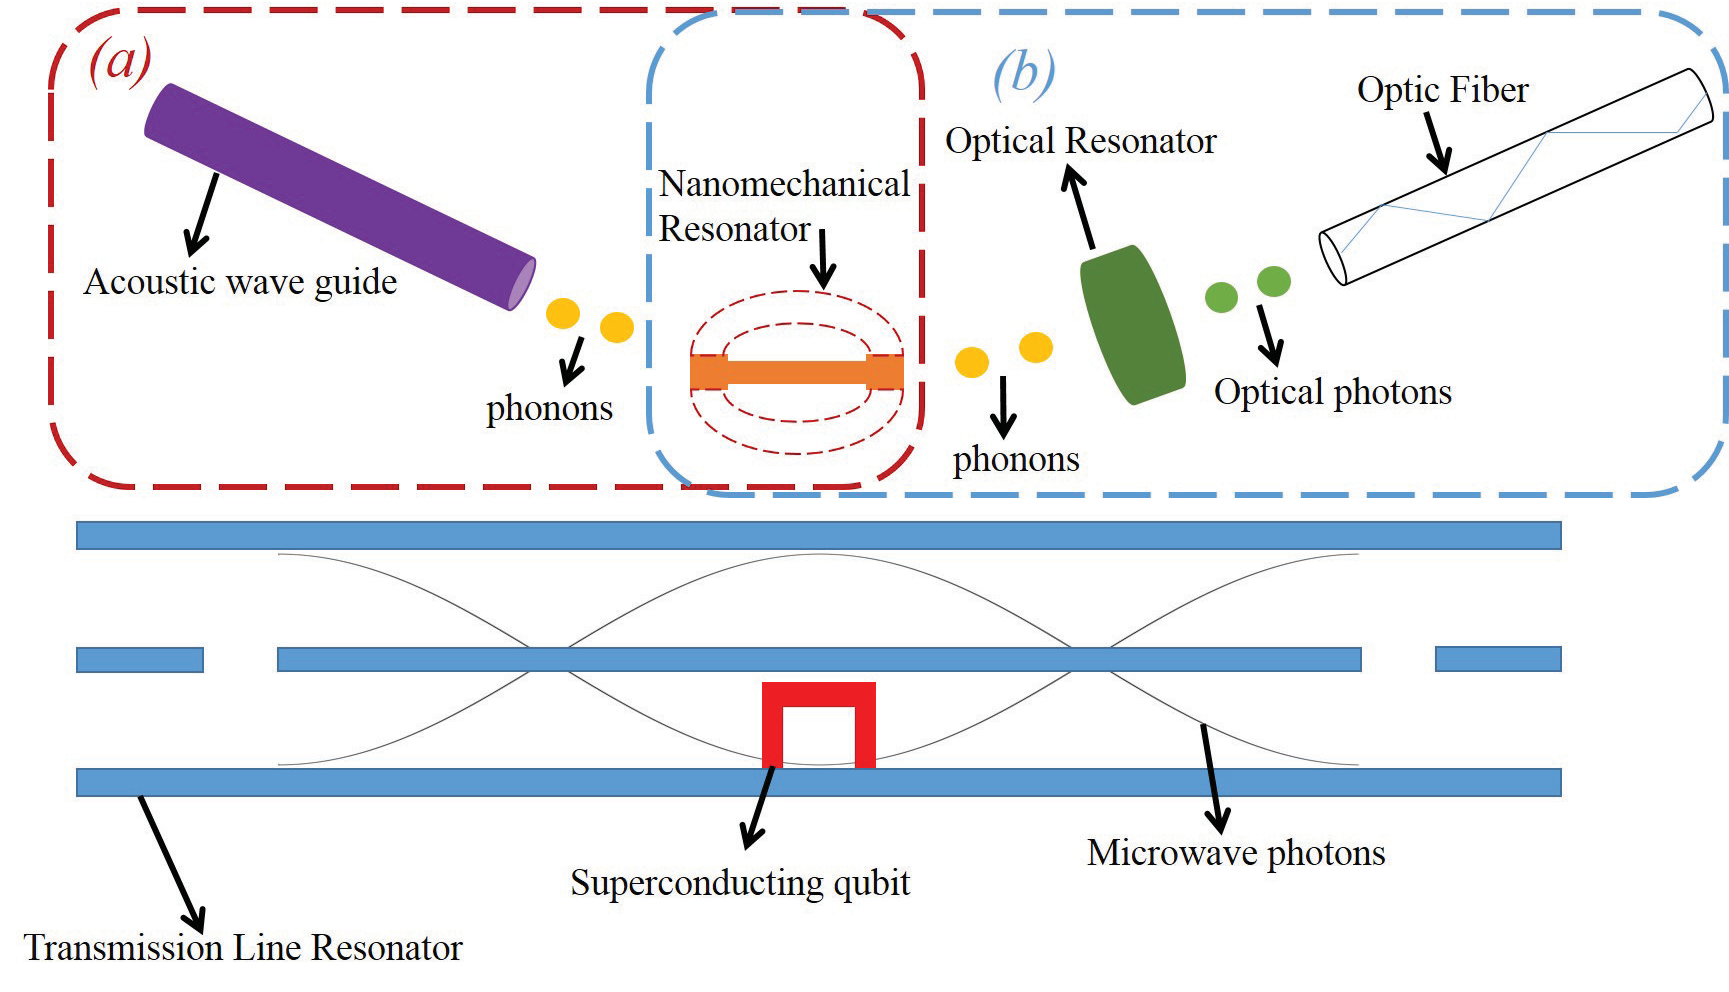
\includegraphics[width=0.475\textwidth]{transducer_scheme_1}
\caption{The scheme of opto-mechanics based quantum transducer is described in the figure above. The various components of the transducer are labeled correspondingly. There are two possible ways of converting the microwaves using opto-mechanics based transducer. The final steps for the process in which acoustic modes are transported using waveguides is enclosed by a brown coloured box with dashed outlines labeled (a). Similarly the blue coloured box labeled (b) represents the scheme where the phonons are converted to optical photons which is then transmitted via optic fibre. The initial few steps consisting of the superconducting qubit, transmission line resonator and microwaves are common to both the processes.}
\end{figure}

\begin{figure}[t]
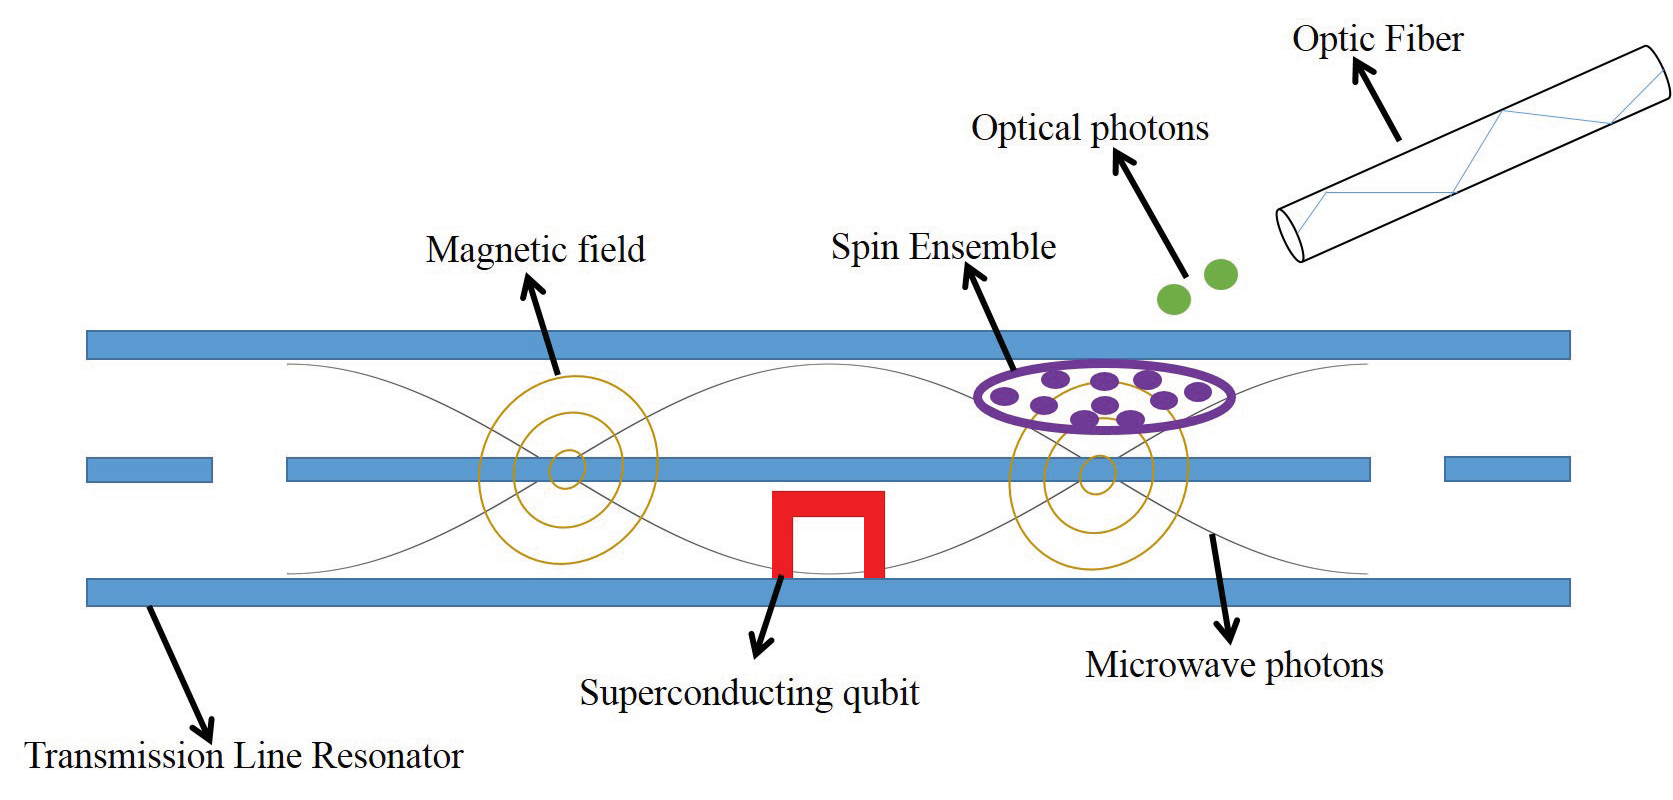
\includegraphics[width=0.475\textwidth]{transducer_scheme_2}
\caption{The spin ensemble based quantum transducer is described in the schematic sketch shown above. The microwave photons are converted to optical photons via a spin ensemble. The different components of the scheme are all labeled appropriately. }
\end{figure}

\bibliography{ref}
 
\end{document}

